\documentclass[12pt,]{article}
\usepackage{lmodern}
\usepackage{amssymb,amsmath}
\usepackage{ifxetex,ifluatex}
\usepackage{fixltx2e} % provides \textsubscript
\ifnum 0\ifxetex 1\fi\ifluatex 1\fi=0 % if pdftex
  \usepackage[T1]{fontenc}
  \usepackage[utf8]{inputenc}
\else % if luatex or xelatex
  \ifxetex
    \usepackage{mathspec}
  \else
    \usepackage{fontspec}
  \fi
  \defaultfontfeatures{Ligatures=TeX,Scale=MatchLowercase}
\fi
% use upquote if available, for straight quotes in verbatim environments
\IfFileExists{upquote.sty}{\usepackage{upquote}}{}
% use microtype if available
\IfFileExists{microtype.sty}{%
\usepackage{microtype}
\UseMicrotypeSet[protrusion]{basicmath} % disable protrusion for tt fonts
}{}
\usepackage[margin=2.5cm]{geometry}
\usepackage{hyperref}
\hypersetup{unicode=true,
            pdftitle={Factors influencing the levels of mercury in the hair of fishermen and non-fishermen},
            pdfauthor={Urvan Christen, Amandine Goffeney, Joseph Vermeil, Lucile Vigué},
            pdfborder={0 0 0},
            breaklinks=true}
\urlstyle{same}  % don't use monospace font for urls
\usepackage{graphicx,grffile}
\makeatletter
\def\maxwidth{\ifdim\Gin@nat@width>\linewidth\linewidth\else\Gin@nat@width\fi}
\def\maxheight{\ifdim\Gin@nat@height>\textheight\textheight\else\Gin@nat@height\fi}
\makeatother
% Scale images if necessary, so that they will not overflow the page
% margins by default, and it is still possible to overwrite the defaults
% using explicit options in \includegraphics[width, height, ...]{}
\setkeys{Gin}{width=\maxwidth,height=\maxheight,keepaspectratio}
\IfFileExists{parskip.sty}{%
\usepackage{parskip}
}{% else
\setlength{\parindent}{0pt}
\setlength{\parskip}{6pt plus 2pt minus 1pt}
}
\setlength{\emergencystretch}{3em}  % prevent overfull lines
\providecommand{\tightlist}{%
  \setlength{\itemsep}{0pt}\setlength{\parskip}{0pt}}
\setcounter{secnumdepth}{0}
% Redefines (sub)paragraphs to behave more like sections
\ifx\paragraph\undefined\else
\let\oldparagraph\paragraph
\renewcommand{\paragraph}[1]{\oldparagraph{#1}\mbox{}}
\fi
\ifx\subparagraph\undefined\else
\let\oldsubparagraph\subparagraph
\renewcommand{\subparagraph}[1]{\oldsubparagraph{#1}\mbox{}}
\fi

%%% Use protect on footnotes to avoid problems with footnotes in titles
\let\rmarkdownfootnote\footnote%
\def\footnote{\protect\rmarkdownfootnote}

%%% Change title format to be more compact
\usepackage{titling}

% Create subtitle command for use in maketitle
\providecommand{\subtitle}[1]{
  \posttitle{
    \begin{center}\large#1\end{center}
    }
}

\setlength{\droptitle}{-2em}

  \title{Factors influencing the levels of mercury in the hair of fishermen and
non-fishermen}
    \pretitle{\vspace{\droptitle}\centering\huge}
  \posttitle{\par}
    \author{Urvan Christen, Amandine Goffeney, Joseph Vermeil, Lucile Vigué}
    \preauthor{\centering\large\emph}
  \postauthor{\par}
      \predate{\centering\large\emph}
  \postdate{\par}
    \date{June 2019}

\usepackage{booktabs}
\usepackage{longtable}
\usepackage{array}
\usepackage{multirow}
\usepackage{wrapfig}
\usepackage{float}
\usepackage{colortbl}
\usepackage{pdflscape}
\usepackage{tabu}
\usepackage{threeparttable}
\usepackage{threeparttablex}
\usepackage[normalem]{ulem}
\usepackage{makecell}
\usepackage{xcolor}

\usepackage{float}
\usepackage{fancyhdr}
\usepackage{wrapfig, subfig}
\pagestyle{fancy}
\fancyhead[LE,RO]{Christen, Goffeney, Vermeil, Vigue}

\begin{document}
\maketitle

\subsection{Introduction}\label{introduction}

Mercury is a metal present in the environment whose harmful effects on
human health are well known
{[}\protect\hyperlink{ref-park2012human}{1}{]}. In \emph{Al-Majed and
Preston} study {[}\protect\hyperlink{ref-al2000factors}{2}{]}, total
mercury and methyl mercury levels in the hair of 100 fishermen of
Kuwait, aged 16 to 58 years, were compared to those of a control
population of 35 non-fishermen, aged 26 to 35 years. The aim of our
study is to analyse the factors influencing the levels of mercury in
both populations. For the sake of simplicity, we will only focus on
total Hg, leaving out methyl mercury, since both variables are strongly
correlated (shown in the paper). The dataset contains six numerical
variables (age, height, weight, number of fish meals per week and
residence time in Kuwait) and two categorical variables (being a
fisherman or not, fish consumption habits). All study participants are
male.

\begin{table}[t]

\caption{\label{tab:unnamed-chunk-6}\label{tbl:fishmlwk}Distribution of the number of fish meals accross fishermen and non-fishermen populations}
\centering
\begin{tabular}{lrrrrrrrr}
\toprule
  & 0 & 1 & 2 & 3 & 4 & 7 & 14 & 21\\
\midrule
\rowcolor{gray!6}  non-fisherman & 10 & 14 & 11 & 0 & 0 & 0 & 0 & 0\\
fisherman & 0 & 0 & 0 & 2 & 12 & 70 & 5 & 11\\
\bottomrule
\end{tabular}
\end{table}

\begin{table}[t]

\caption{\label{tab:unnamed-chunk-7}\label{tbl:correlation}Correlation matrix}
\centering
\begin{tabular}{l|r|r|r|r|r|r|r|r}
\hline
  & fisherman & age & restime & height & weight & fishmlwk & fishpart & TotHg\\
\hline
\rowcolor{gray!6}  fisherman & 1.00 & 0.25 & 0.25 & -0.06 & -0.09 & 0.61 & 0.46 & 0.23\\
\hline
age & 0.25 & 1.00 & 0.58 & 0.00 & 0.05 & 0.26 & -0.01 & 0.16\\
\hline
\rowcolor{gray!6}  restime & 0.25 & 0.58 & 1.00 & -0.05 & 0.11 & 0.19 & 0.00 & 0.06\\
\hline
height & -0.06 & 0.00 & -0.05 & 1.00 & 0.30 & -0.04 & -0.03 & 0.19\\
\hline
\rowcolor{gray!6}  weight & -0.09 & 0.05 & 0.11 & 0.30 & 1.00 & 0.04 & -0.05 & 0.41\\
\hline
fishmlwk & 0.61 & 0.26 & 0.19 & -0.04 & 0.04 & 1.00 & 0.19 & 0.30\\
\hline
\rowcolor{gray!6}  fishpart & 0.46 & -0.01 & 0.00 & -0.03 & -0.05 & 0.19 & 1.00 & 0.11\\
\hline
TotHg & 0.23 & 0.16 & 0.06 & 0.19 & 0.41 & 0.30 & 0.11 & 1.00\\
\hline
\end{tabular}
\end{table}

\subsection{Exploratory analysis}\label{exploratory-analysis}

Before fitting a model, we first look at the data. Table
\ref{tbl:fishmlwk} shows the distribution of individuals according to
the number of fish meals per week and the two groups. We note that for
some values, there are very few people. For instance, only two people
eat fish three times per week. We also see that the number of fish meals
per week is completely separable by population group. This is quantified
and illustrated by the correlation matrix (Table \ref{tbl:correlation})
and the pair plots (Figure \ref{fig:pair_plots}). They reveal the strong
correlation observed between \emph{fisherman} and \emph{fishmlwk}.
Moreover other expected correlations appear, between \emph{height} and
\emph{weight} or \emph{age} and \emph{restime} especially, but they stay
quite weak. To quantify this multicolinearity of variables, we use the
variance inflation factor (VIF). We set the following criterion: we keep
only the variables that have a result below 5. We observe that all the
variables have a variance inflation factor below 2, so we do not
eliminate any variable, for the moment.

\begin{figure}[htbp]

{\centering 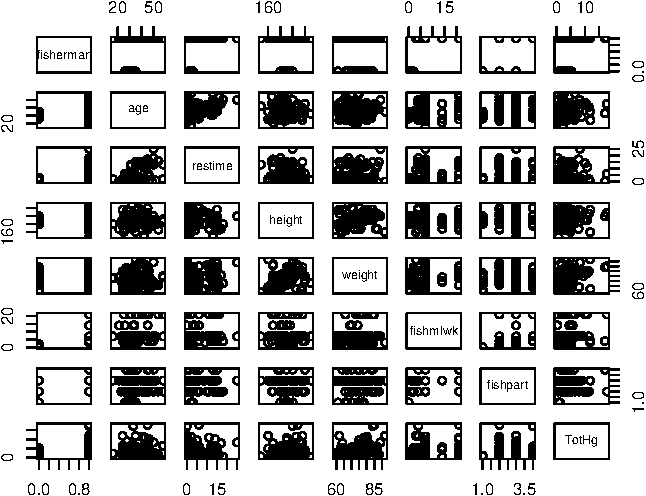
\includegraphics{Report_files/figure-latex/unnamed-chunk-8-1} 

}

\caption{\label{fig:pair_plots}Pair plots}\label{fig:unnamed-chunk-8}
\end{figure}

\subsection{Model selection}\label{model-selection}

We now use a stepwise method of model selection to select the more
relevant variables to explain the \emph{TotHg} variations within the
population. The selection of the model is based on the AIC score of the
model, which means that after having added or deleted an explanatory
variable from the model, the algorithm keeps the new model if the AIC
score is better. In the end, it is an optimisation problem in which we
want to find the model with the lowest possible AIC score. We begin our
process of model selection with a formula with all the variables to the
first order. After this stepwise selection, the selected model is:

\begin{equation}
\label{eqn:fullmodel}
\begin{split}
TotHg = \beta_0 + \beta_1 \cdot fisherman  + \beta_2 \cdot age + \beta_3 \cdot restime + \beta_4 \cdot weight + \beta_5 \cdot fishmlwk
\end{split}
\end{equation}

(Table \ref{tbl:fullmodel}). The intercept and the weight coefficient
are highly significant but the others are not. However, the signs of the
coefficients are not absurd: while it is not really intuitive that the
weight coefficient should be positive or negative, the coefficient of
\emph{fishmlwk} has to be positive, and it is the case here. Now, to
determine possible differences between the fishermen and non-fishermen,
a model based on the interactions between the \emph{fisherman} variable
and all the others is proposed. The best model is now given by model
\ref{eqn:interactionmodel} with estimates in Table
\ref{tbl:interactionmodel}.

\begin{equation}
\label{eqn:interactionmodel}
\begin{split}
TotHg = &\beta_0 + \beta_1 \cdot fisherman + \beta_2 \cdot weight +  \beta_3 \cdot fishmlwk \\&+ \beta_4 \cdot fisherman \cdot weight + \beta_5 \cdot fisherman \cdot fishmlwk
\end{split}
\end{equation}

\begin{table}[t]

\caption{\label{tab:unnamed-chunk-12}\label{tbl:fullmodel}First order model regression results}
\centering
\begin{tabular}{l|l|l|l|l}
\hline
  & Estimate & Std. Error & t value & Pr(>|t|)\\
\hline
\rowcolor{gray!6}  (Intercept) & -12.68 & 2.71 & -4.68 & 7.0e-06\\
\hline
fisherman & 1.11 & 0.65 & 1.70 & 9.1e-02\\
\hline
\rowcolor{gray!6}  age & 0.05 & 0.03 & 1.43 & 1.6e-01\\
\hline
restime & -0.08 & 0.05 & -1.45 & 1.5e-01\\
\hline
\rowcolor{gray!6}  weight & 0.19 & 0.03 & 5.58 & 1.4e-07\\
\hline
fishmlwk & 0.10 & 0.05 & 1.82 & 7.2e-02\\
\hline
\end{tabular}
\end{table}

\begin{table}[t]

\caption{\label{tab:unnamed-chunk-14}\label{tbl:interactionmodel}Final model regression results}
\centering
\begin{tabular}{l|l|l|l|l}
\hline
  & Estimate & Std. Error & t value & Pr(>|t|)\\
\hline
\rowcolor{gray!6}  (Intercept) & -1.42 & 6.94 & -0.20 & 8.4e-01\\
\hline
fisherman & -9.00 & 7.43 & -1.21 & 2.3e-01\\
\hline
\rowcolor{gray!6}  weight & 0.03 & 0.10 & 0.33 & 7.4e-01\\
\hline
fishmlwk & 1.53 & 0.70 & 2.18 & 3.1e-02\\
\hline
\rowcolor{gray!6}  fisherman:weight & 0.16 & 0.11 & 1.48 & 1.4e-01\\
\hline
fisherman:fishmlwk & -1.43 & 0.70 & -2.04 & 4.4e-02\\
\hline
\end{tabular}
\end{table}

\subsection{Results and discussion}\label{results-and-discussion}

We now turn to discussing the results of model
(\ref{eqn:interactionmodel}).

The corresponding coefficients and levels of significance are presented
in Table \ref{tbl:interactionmodel}. What appears is that fishermen have
a basal -9.00 mg/g Hg compared to non-fishermen. Then, \emph{weight} has
a high impact in fishermen: \(\beta_2+\beta_4 = 0.19\), whereas in non
fishermen case only \(\beta_2 = 0.03\) remains. Conversely,
\emph{fishmlwk} is the factor with the highest impact for non-fishermen:
\(\beta_3 = 1.53\) whereas for fishermen \(\beta_3+\beta_5 = 0.1\). In
terms of signifiance only the coefficient concerning \emph{fishmlwk}
appears really reliable.

\subsubsection{Difference between fisherman and control
populations}\label{difference-between-fisherman-and-control-populations}

As described previously, being a fisherman or not has an impact on how
other variables such as \emph{weight} or \emph{fishmlwk} are correlated
to total Hg levels. But in particular this value of \(\beta_1 = -9.00\),
corresponding to \emph{fisherman} variable, is surprising: it seems
counter intuitive that fishermen have 9.00 mg/g Hg less than
non-fishermen. Yet this is compensated by the increased value of
\emph{fisherman:weight}, which will make the overall Hg concentration
more important among fishermen, as expected.

\subsubsection{Number of fish meals per
week}\label{number-of-fish-meals-per-week}

The negative value of \(\beta_5\), corresponding to
\emph{fisherman}:\emph{fishmlwk} interaction, is also surprising: it
suggests that among fishermen the number of fish meals per week has a
weak impact on total Hg levels (\(\beta_3+\beta_5 = 0.1\)) while it has
a much stronger impact on non-fishermen (\(\beta_3 = 1.53\)). However,
previous exploration of data showed that the number of fish meals per
week is completely separable by population group. A simple explanation
could be that the relation between the number of fish meals per week and
total Hg levels is positive but not linear: it increases fast for low
numbers of fish meals (i.e.~for non-fishermen) and more slowly for high
numbers of fish meals (i.e.~for fishermen). Furthermore, the observable
does not reflect entirely the quantity of fish eaten, since one can eat
more or less fish per meal. The weight of fish eaten per week might be a
more accurate observable to study.

\subsubsection{Weight}\label{weight}

The positive influence of weight on this concentration was unexpected,
since a concentration and not an absolute quantity was measured. However
it could have many possible explanations. Weight is much likely
correlated with adiposity, and adipose tissue more susceptible to retain
toxins than others. Another explanation could be that the fatter, the
more one eats and possibly ingests mercury that could fix in the hair;
since body weight is probably not correlated with the amount of hair, it
could explain the high mercury concentration in hair.

\subsubsection{Diagnostic plots}\label{diagnostic-plots}

\begin{figure}[htbp]

{\centering \subfloat[\label{fig:residuals}residuals\label{fig:unnamed-chunk-181}]{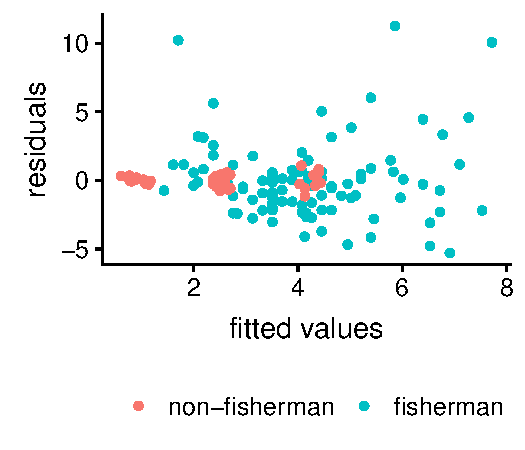
\includegraphics[width=.7\linewidth,height=7cm]{Report_files/figure-latex/unnamed-chunk-18-1} }\subfloat[\label{fig:QQ}QQ-plot\label{fig:unnamed-chunk-182}]{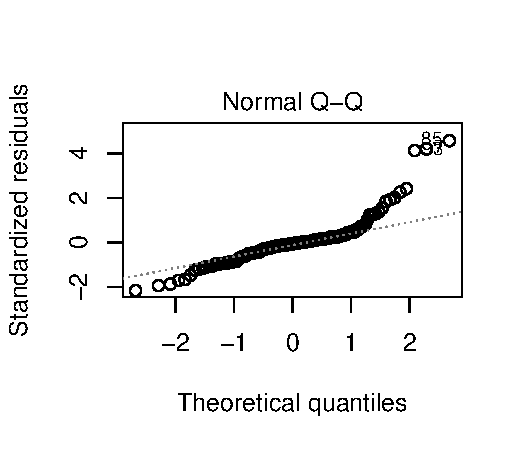
\includegraphics[width=.7\linewidth,height=7cm]{Report_files/figure-latex/unnamed-chunk-18-2} }

}

\caption{Diagnostic plots}\label{fig:unnamed-chunk-18}
\end{figure}

The plot of the residuals against the fitted values (Figure
\ref{fig:residuals}) helps us to assess three assumptions about the
residuals. First, the mean of the residuals should be 0, and the plot
confirms it. Second, the model should be homoscedastic, but the plot
tends to show it is not the case. Indeed, a model is homoscedastic if
the variance is the same for all the values, and here, the variance is
much higher for fishermen than for non-fishermen. However, within each
class, the variance is overall similar, even if it tends to be a little
more spread for high fitted values. Eventually the uncorrelation between
the X variables and the residuals is again confirmed by the plot.

The QQ plot shows that we have a heavy tailed distribution of residuals,
with a very heavy right tail. It could be explained by a non-linear
relation between the variables and the concentration of mercury.

\subsection{Conclusion}\label{conclusion}

We have built a simple model that can help to explain the levels of
mercury observed in a fishermen population compared to a control group.
It appears that the variables having the most significant influence over
the measured levels of mercury are the weight of the individual and the
frequency at which they eat fish. The former can seem surprising even
though some hypotheses can be formed to account for the influence of
weight on mercury levels. The latter may be the main explanation for the
differences observed between our two groups: fishermen eat fish much
more often than non-fishermen, since fish is a well-known source of
mercury it seems logical to see a positive correlation between fish meal
frequency and mercury levels and thus to observe higher mercury levels
in fishermen populations compared to non-fishermen.

\subsection*{References}\label{references}
\addcontentsline{toc}{subsection}{References}

\hypertarget{refs}{}
\hypertarget{ref-park2012human}{}
{[}1{]} J.-D. Park and W. Zheng, ``Human exposure and health effects of
inorganic and elemental mercury,'' \emph{Journal of preventive medicine
and public health}, vol. 45, no. 6, p. 344, 2012.

\hypertarget{ref-al2000factors}{}
{[}2{]} N. Al-Majed and M. Preston, ``Factors influencing the total
mercury and methyl mercury in the hair of the fishermen of kuwait,''
\emph{Environmental Pollution}, vol. 109, no. 2, pp. 239--250, 2000.


\end{document}
